\documentclass{article}
\usepackage[utf8]{inputenc}
\usepackage{hyperref}
\usepackage{pdfpages}
\usepackage{graphicx}
\usepackage{textcomp}
\usepackage{listings}
\usepackage[parfill]{parskip}
\usepackage{wrapfig}


\graphicspath{ {resources/images/} }

\title{Understand CPM and run examples in Compucell3D}
\author{unsupo }
\date{October 2016}

\hypersetup{colorlinks=true,urlcolor=blue}

\begin{document}

\maketitle

\tableofcontents

\section{Problem Statement}
Here is an excellent tutorial to go through to understand the theory of the Cellular Potts Model and its implementation in 
\href{http://www.compucell3d.org/BinDoc/cc3d_binaries/Manuals/Introduction_To_CompuCell3D_v.3.6.2.pdf}{Introduction To CompuCell3D}

In this assignment, you are to go through the tutorial, download, install compucell 3D and run the example systems. Specifically, run the cell sorting instance and understand the relationship between the different values of cell type adhesion and the resulting cellular morphology.

Write a short report that describes your experiments modifying the values of adhesion and provide examples of the final cellular patterns.

\newpage
\section{Installing and Running Compucell 3D}
To install Compucell 3D on Mac 10.11.x follow this link \href{https://sourceforge.net/projects/cc3d/files/3.7.5/mac/elcapitan-10.11/}{Compucell3D Download}

Unzip the resultant download.  Inside the unzipped directory run a file called \textbf{compucell3d.command}.  This will open up compucell3d.

{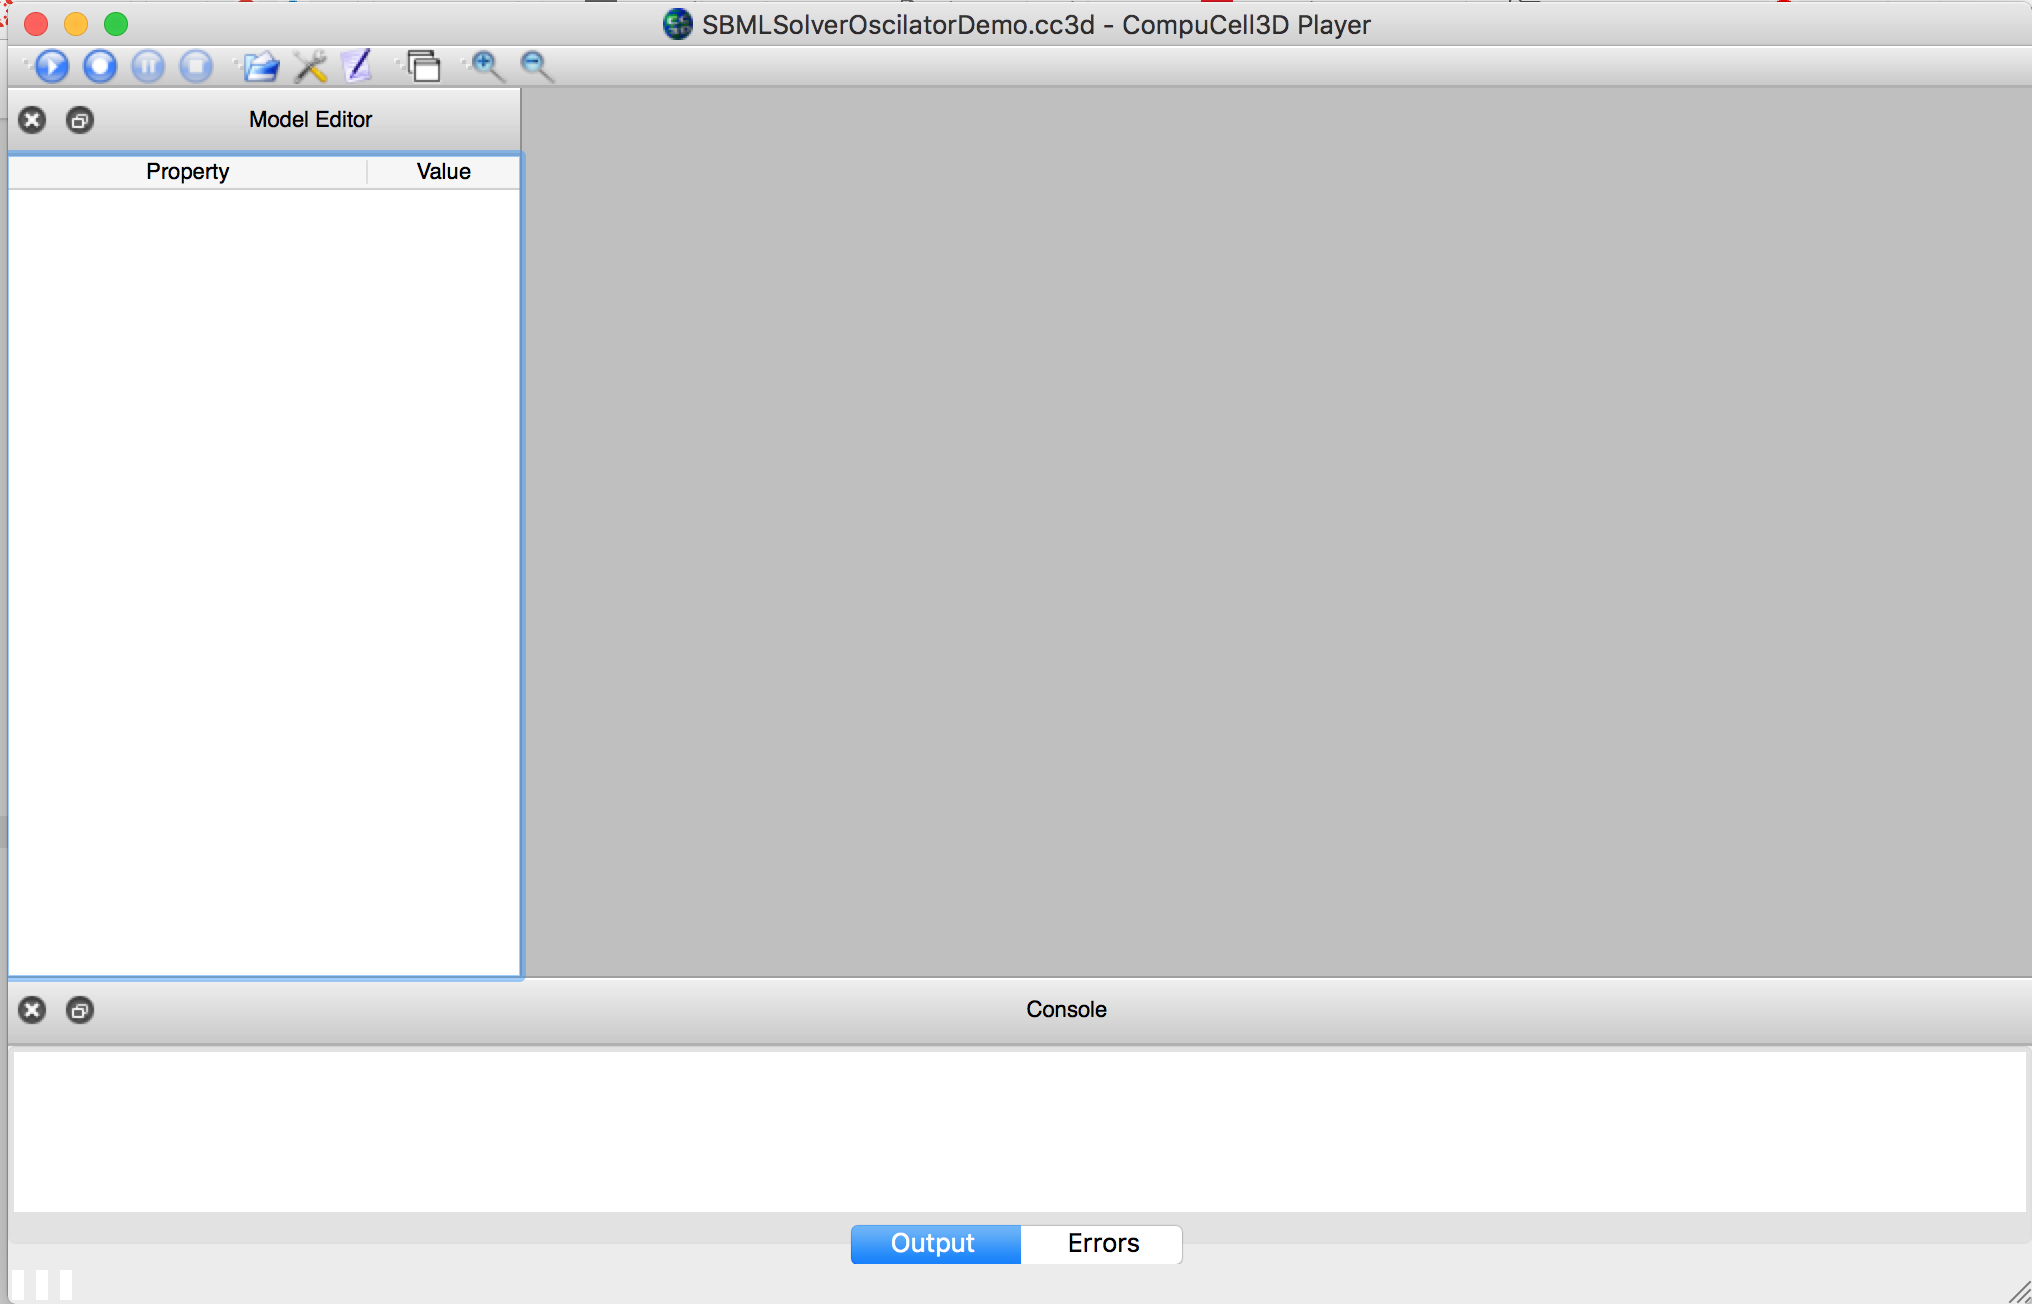
\includegraphics[width=\textwidth]{compucell3d}
\centering}

Then under file \textrightarrow Open Simulation File (.cc3d) \textless command\textgreater O
The demo files are under the Demos directory, open the Demos/Models/cellsort/cellsort\textunderscore 2D/cellsort\textunderscore 2D.cc3d

\newpage
After clicking the play button or Simulation \textrightarrow Run \textless command\textgreater M and letting the simulation run for a minute or two, the simulation will stop on it's own after 9990 steps and produce this output.

{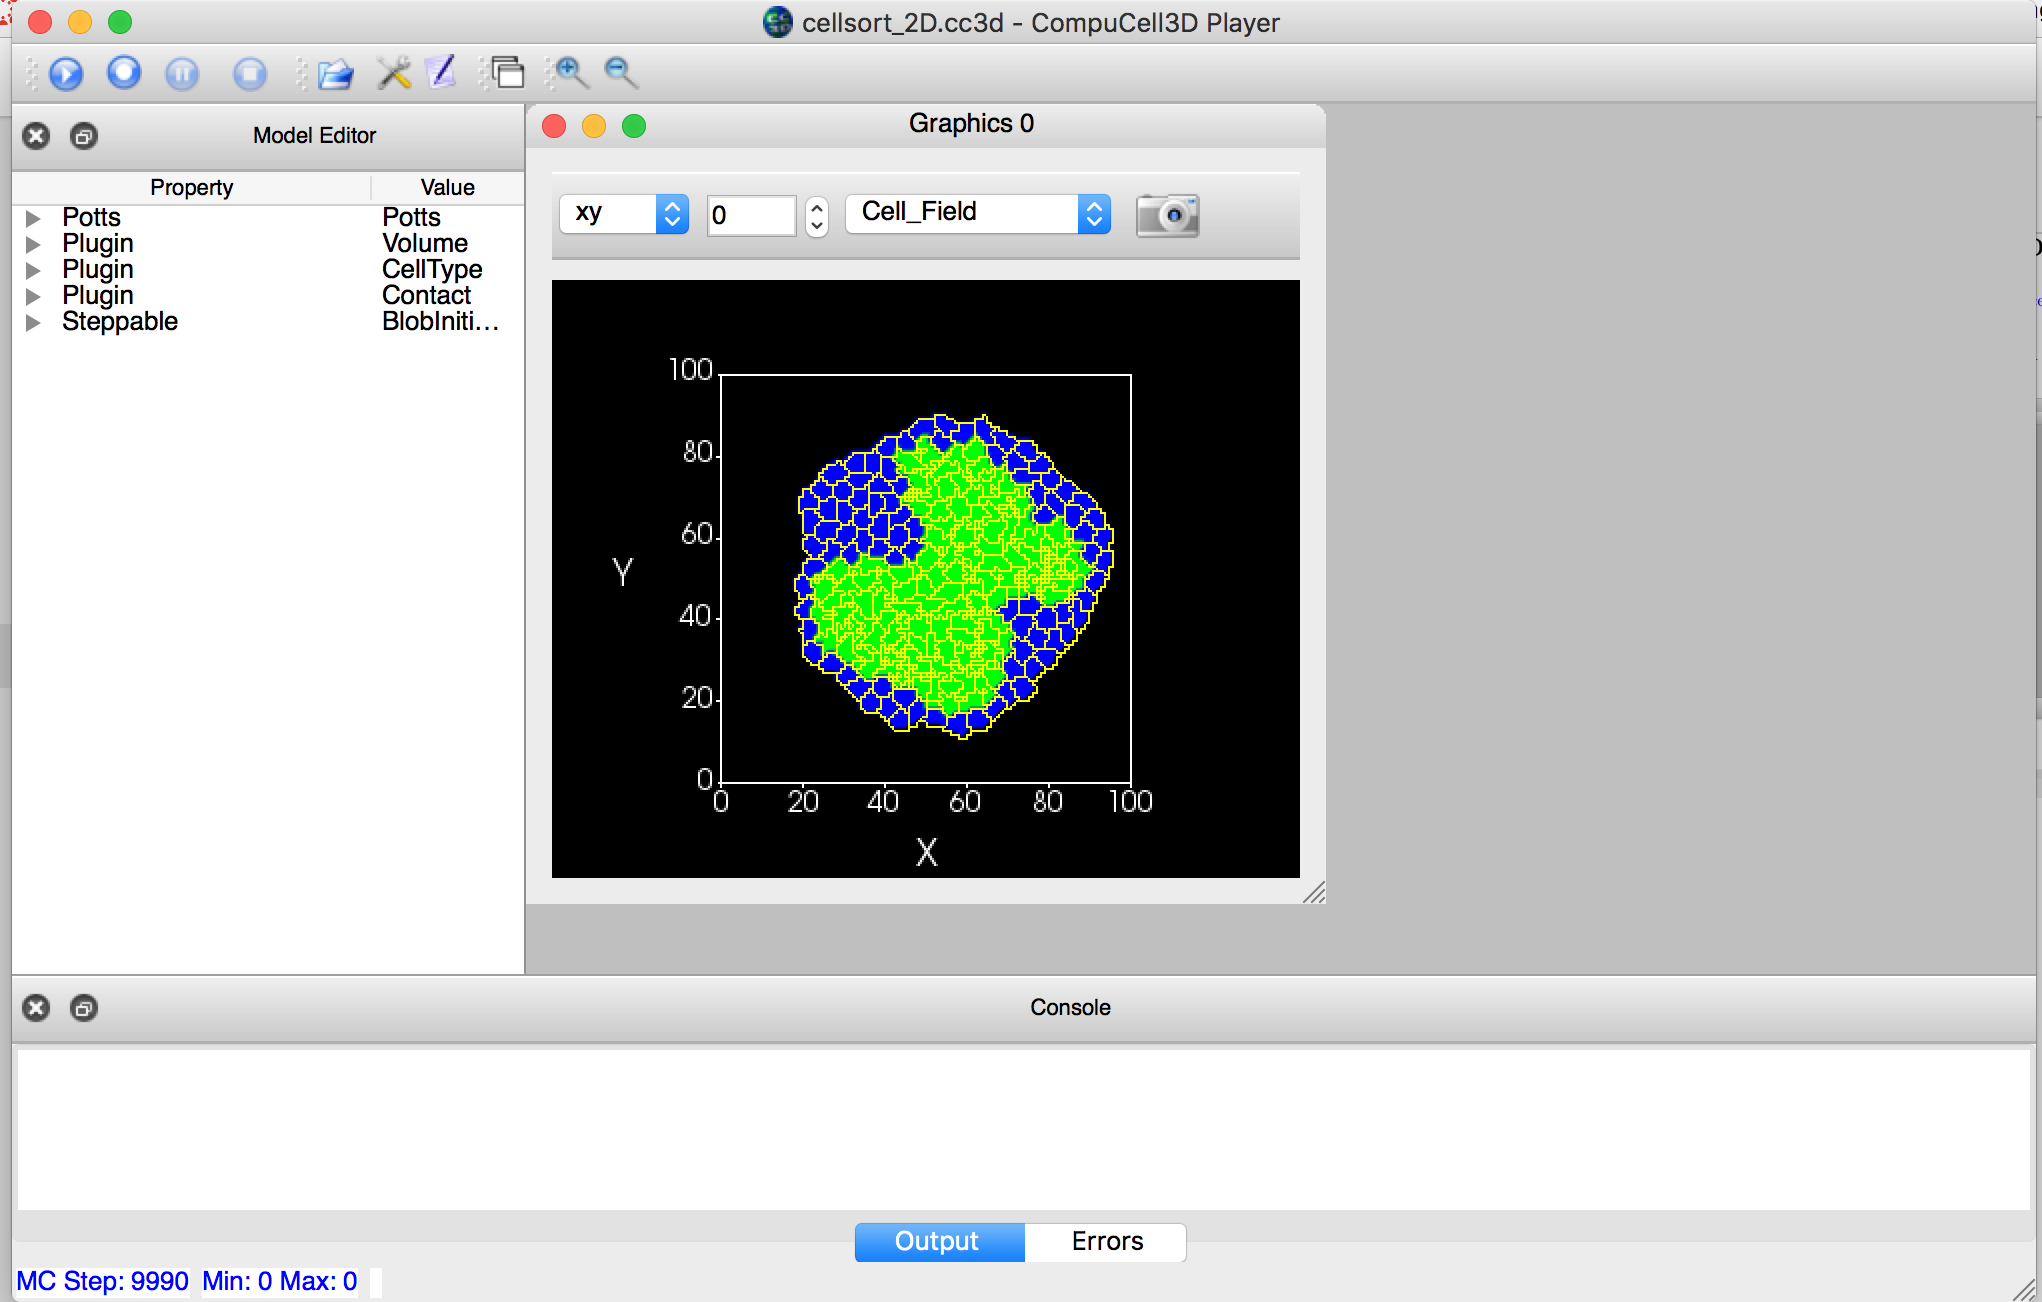
\includegraphics[width=\textwidth]{cellsort2d}
\centering}

\newpage
\section{Modifying Values of Adhesion}
Inside the cc3d file used in the simulation shows this:
\lstset{language=XML}
\begin{lstlisting}
<Simulation version="3.6.1">

    <XMLScript Type="XMLScript">Simulation/cellsort_2D.xml</XMLScript>

</Simulation>
\end{lstlisting}

This points to another xml file which looks like this:
\lstset{language=XML}
\begin{lstlisting}
 <CompuCell3D>
 <Potts>
   <Dimensions x="100" y="100" z="1"/>
   <Anneal>10</Anneal>
   <Steps>10000</Steps>
   <Temperature>10</Temperature>
   <Flip2DimRatio>1</Flip2DimRatio>
   <NeighborOrder>2</NeighborOrder>
 </Potts>


 <Plugin Name="Volume">
   <TargetVolume>25</TargetVolume>
   <LambdaVolume>2.0</LambdaVolume>
 </Plugin>

<Plugin Name="CellType">
    <CellType TypeName="Medium" TypeId="0"/>
    <CellType TypeName="Condensing" TypeId="1"/>
    <CellType TypeName="NonCondensing" TypeId="2"/>
 </Plugin>

 <Plugin Name="Contact">
   <Energy Type1="Medium" Type2="Medium">0</Energy><!--0-->
   <Energy Type1="NonCondensing" Type2="NonCondensing">16</Energy><!--16-->
   <Energy Type1="Condensing"    Type2="Condensing">2</Energy><!--2-->
   <Energy Type1="NonCondensing" Type2="Condensing">11</Energy><!--11-->
   <Energy Type1="NonCondensing" Type2="Medium">1</Energy><!--16-->
   <Energy Type1="Condensing"    Type2="Medium">1</Energy><!--16-->
   <NeighborOrder>2</NeighborOrder>
 </Plugin>

<Steppable Type="BlobInitializer">
   
   <Region>
      <Center x="50" y="50" z="0"/>
      <Radius>40</Radius>
      <Gap>0</Gap>
      <Width>5</Width>
      <Types>Condensing,NonCondensing</Types>
   </Region>
</Steppable>


</CompuCell3D>

\end{lstlisting}

By modifying the Child elements of the Plugin Name=Contact tag and changing the tex quantity of each of the energy tags, different patterns will be constructed in the cell sorting simulation.

\subsection{Changing Medium Energy}
By changing all the Medium Energy to zero the overall structure seems to explode out.
\begin{figure}[h]
    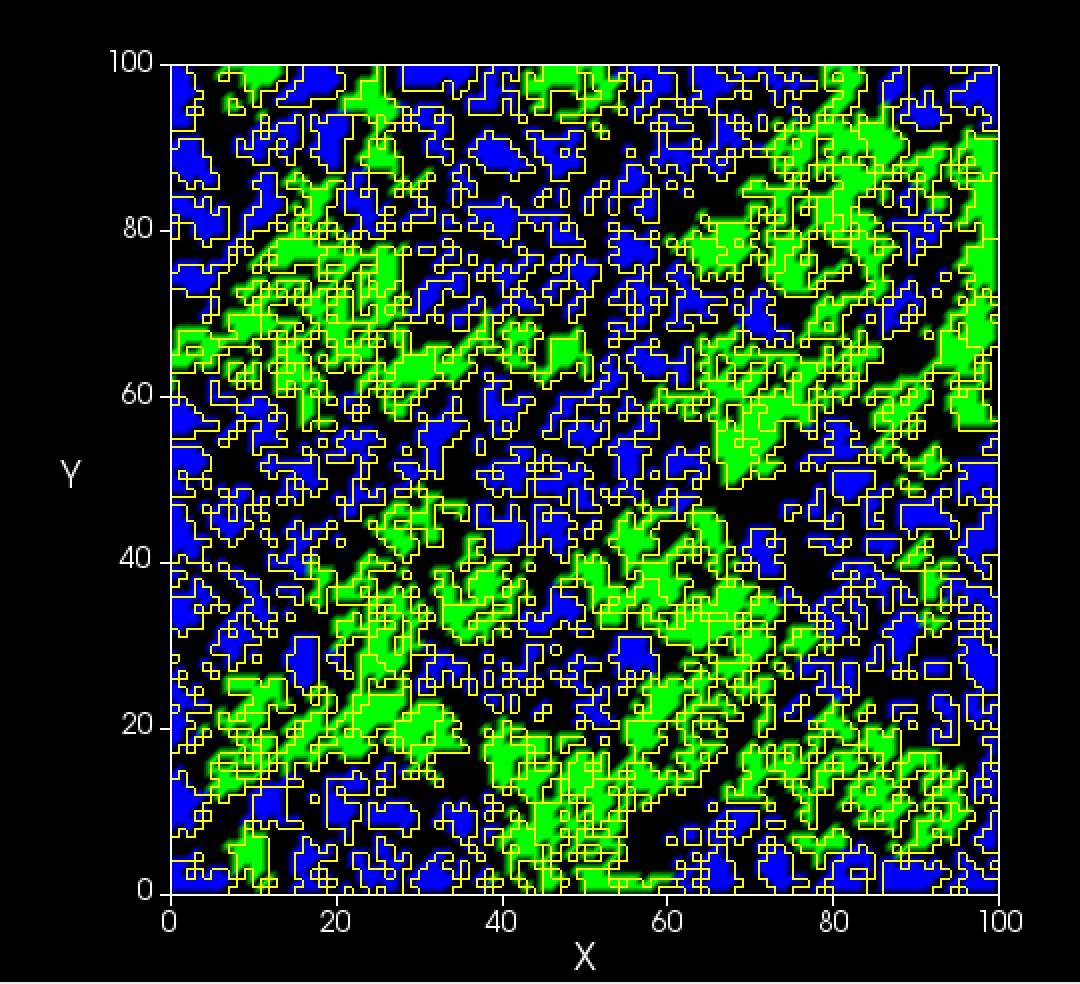
\includegraphics[width=0.5\textwidth]{changing_medium_0s}
\end{figure}
Next is an iteration of making most 0 and each list item value will be set to 100 in the xml.  This should show off any limiting behaviors.

\subsubsection{Medium, Medium}
value = 100.  Medium, Medium appears to not do much as far as the final picture looks like.
    {\centering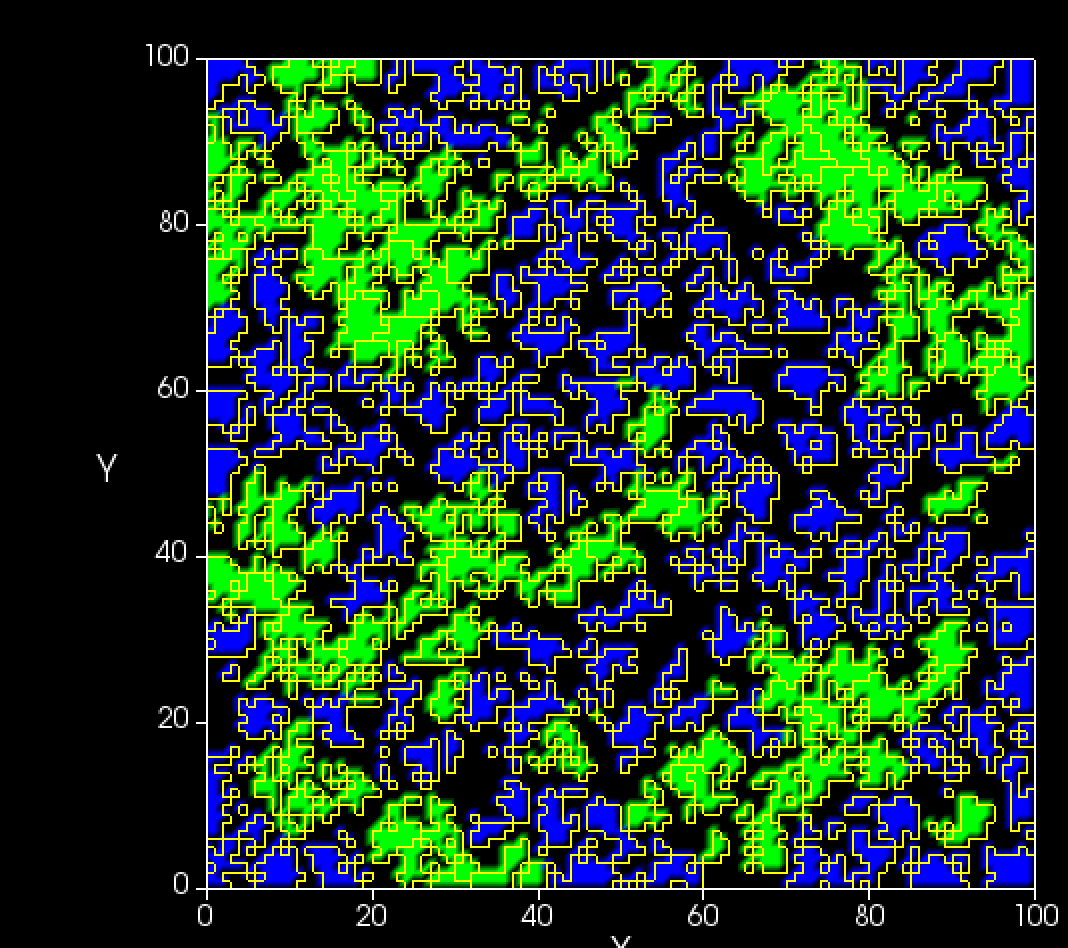
\includegraphics[width=0.5\textwidth]{medium_medium100}}
    
\subsubsection{Medium, NonCondensing}
value = 100. This appears to make the blue clob together, but allow the yellow to scatter.  
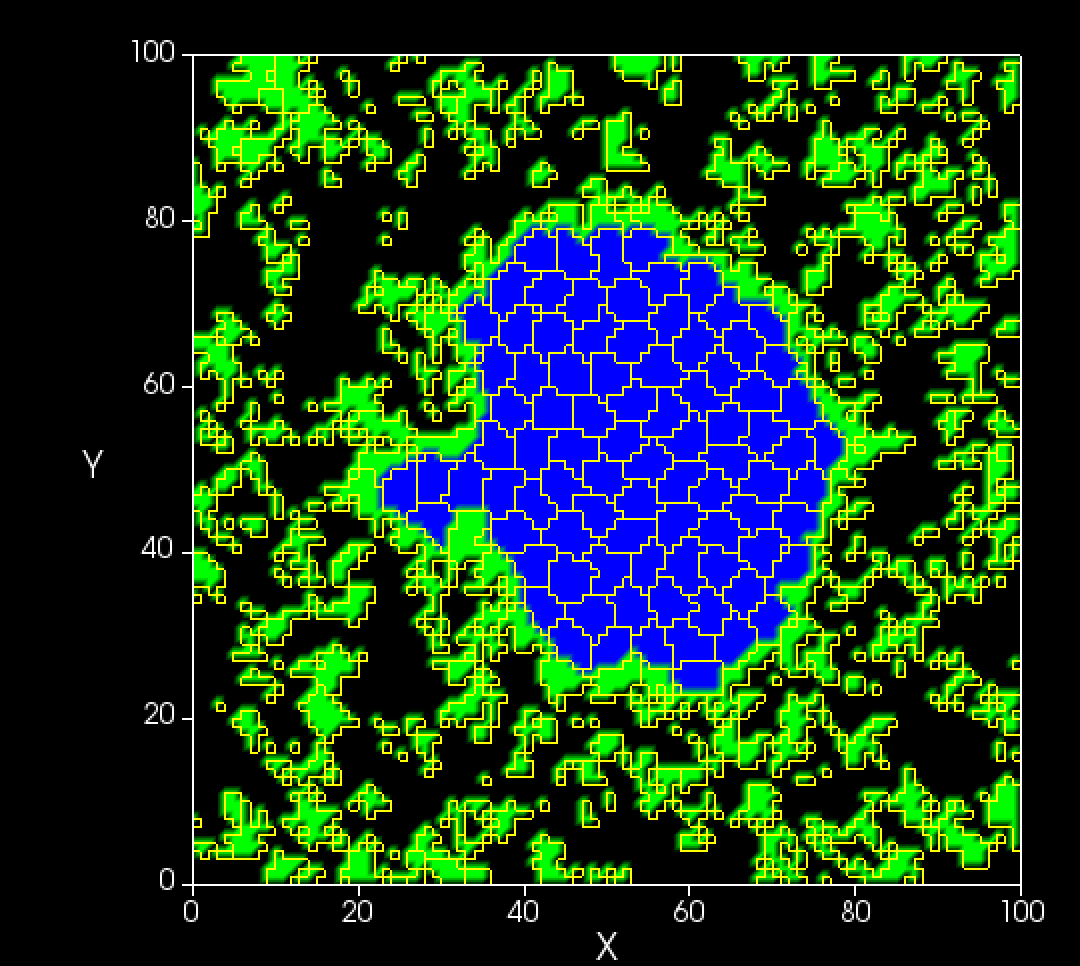
\includegraphics[width=0.5\textwidth]{medium_nonceondensing100}

\subsubsection{Medium, Condensing}
value = 100. This has the opposite effect as above, the blue scatters but the yellow sticks together.  Interesting that a blue clog has appeared inside the yellow.
    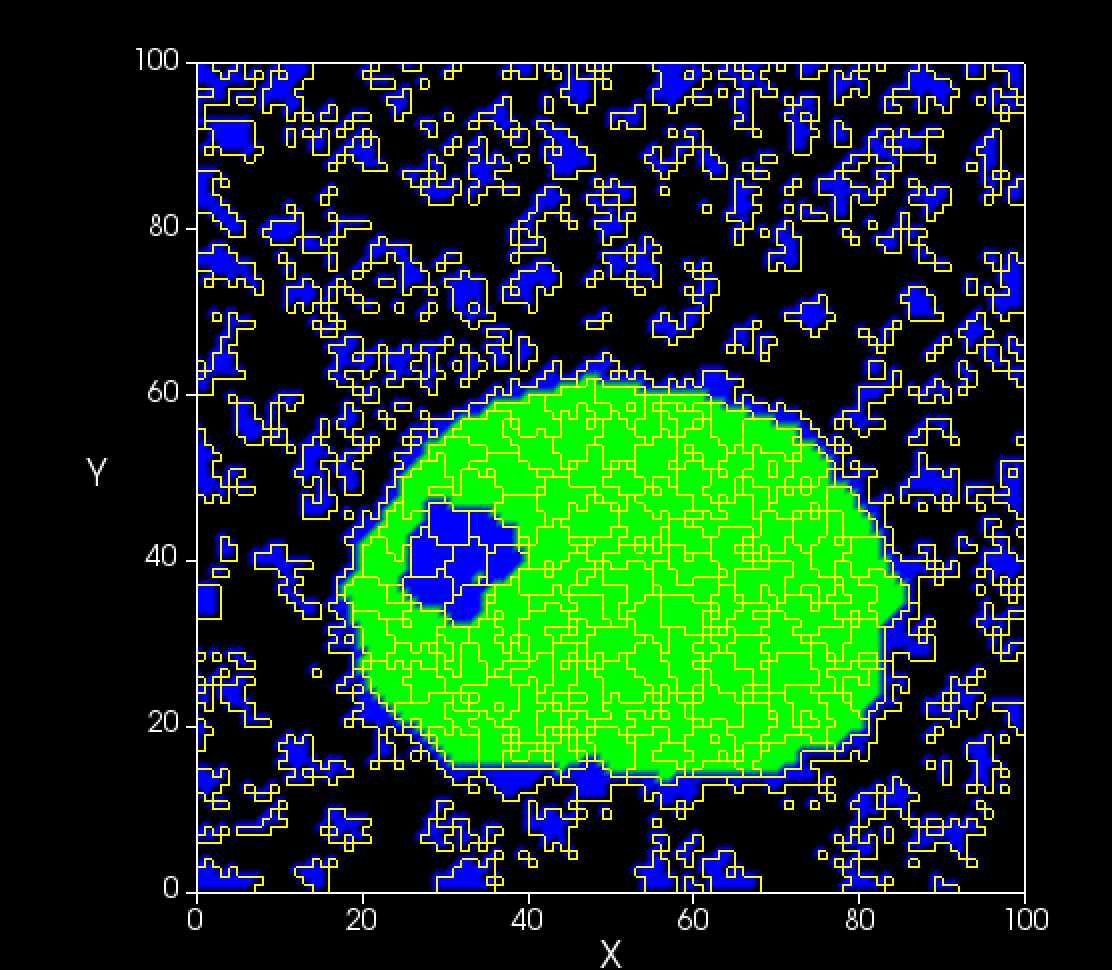
\includegraphics[width=0.5\textwidth]{medium_condensing100}

\subsubsection{Medium, Medium and Medium, NonCondensing}
value = 100.  I stand by my claim that Medium,Medium doesn't do much as this image looks like Medium, NonCondensing alone.  Granted a yellow blob has appeared in the middle, i think this is mere coincidence.
    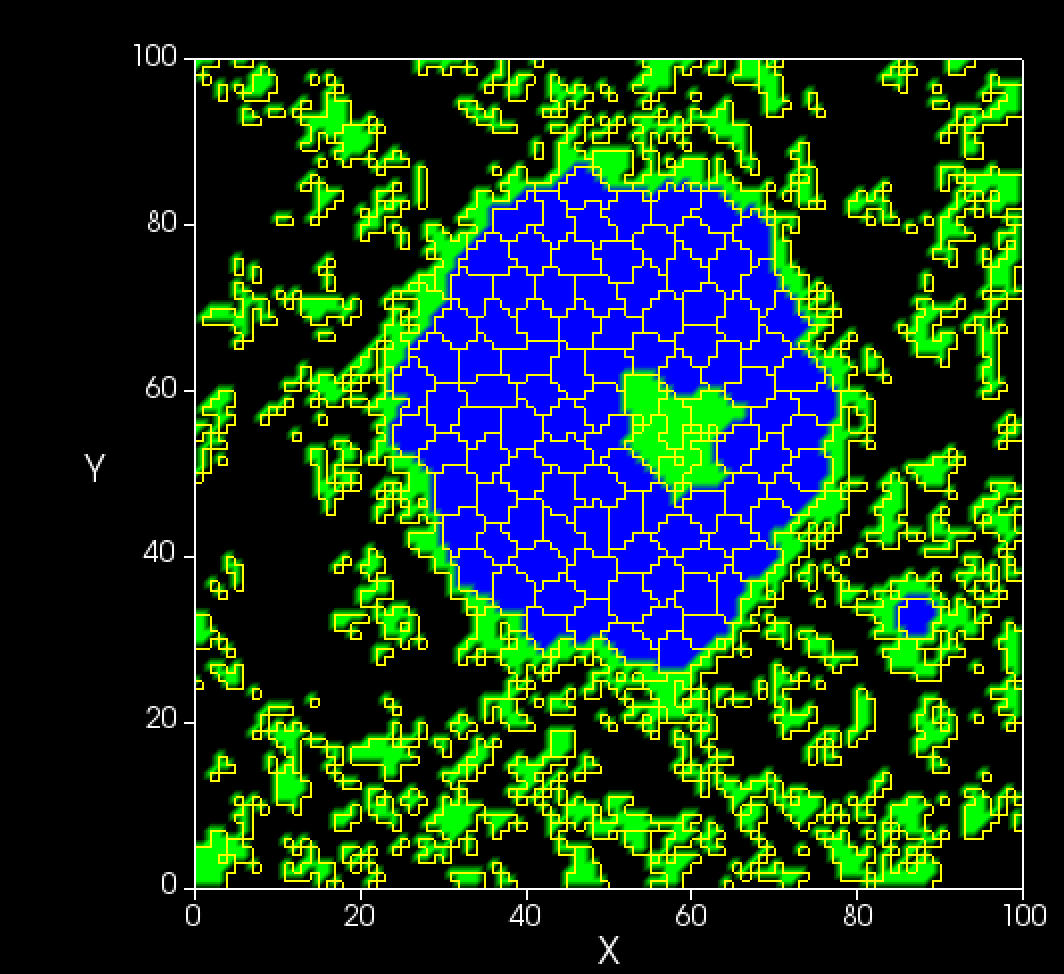
\includegraphics[width=0.5\textwidth]{mm_mnC100}
    
\subsubsection{Medium, Medium and Medium, Condensing}
value = 100.  I stand by my claim that Medium,Medium doesn't do much as this image looks like Medium, Condensing alone.  However the blue blob is larger in the center.  It is possible that the medium medium value determines how much of a blob will appear in the center of the figure
    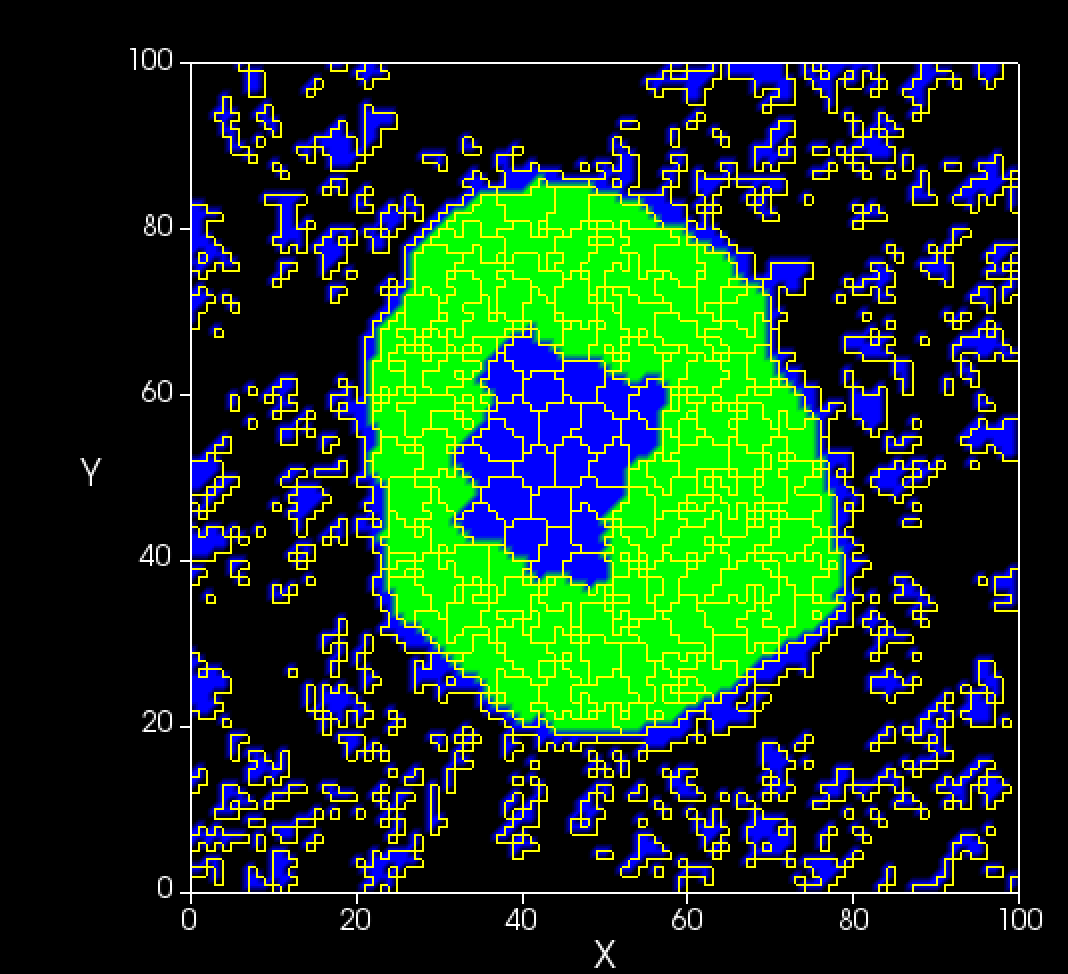
\includegraphics[width=0.5\textwidth]{mm_mc100}

\subsubsection{Medium, Medium, Medium, Condensing and Medium, NonCondensing}
value = 100.  This looks identical to the default value.  Likes like amplifying everything medium doesn't make a huge difference.  However it appeared to converge to a stable state much quicker.  This also created an octogonal pattern.
    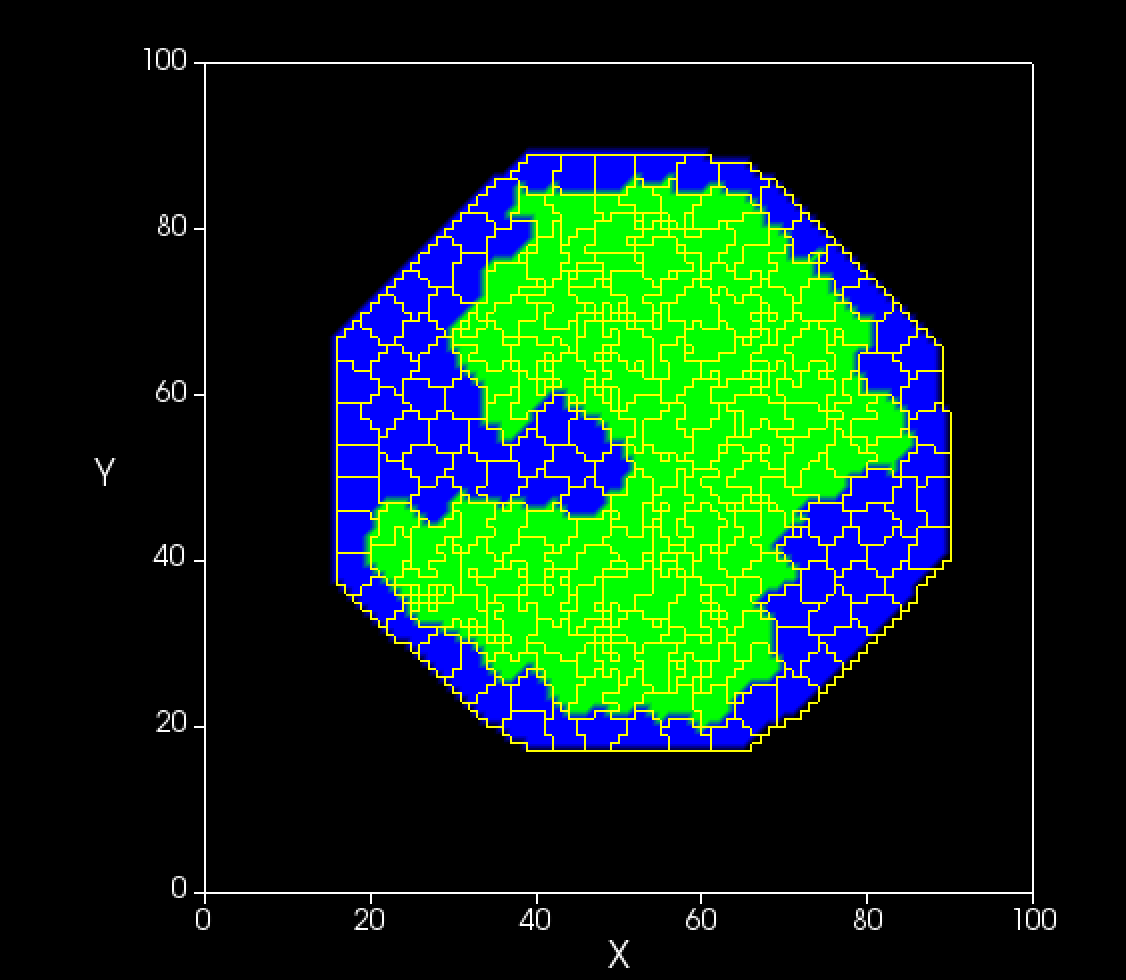
\includegraphics[width=0.5\textwidth]{mm_mc_mnC100}


\subsection{Changing Condensing NonCondensing Energy}
Setting NonCondensing, NonCondensing,, Condensing, Condensing,, and NonCondensing, Condensing to 0 and leaving everything else default results in this image.  Oddly enough it appears to move up and out with these configurations.  No sorting seemed to take place
\begin{figure}[h]
    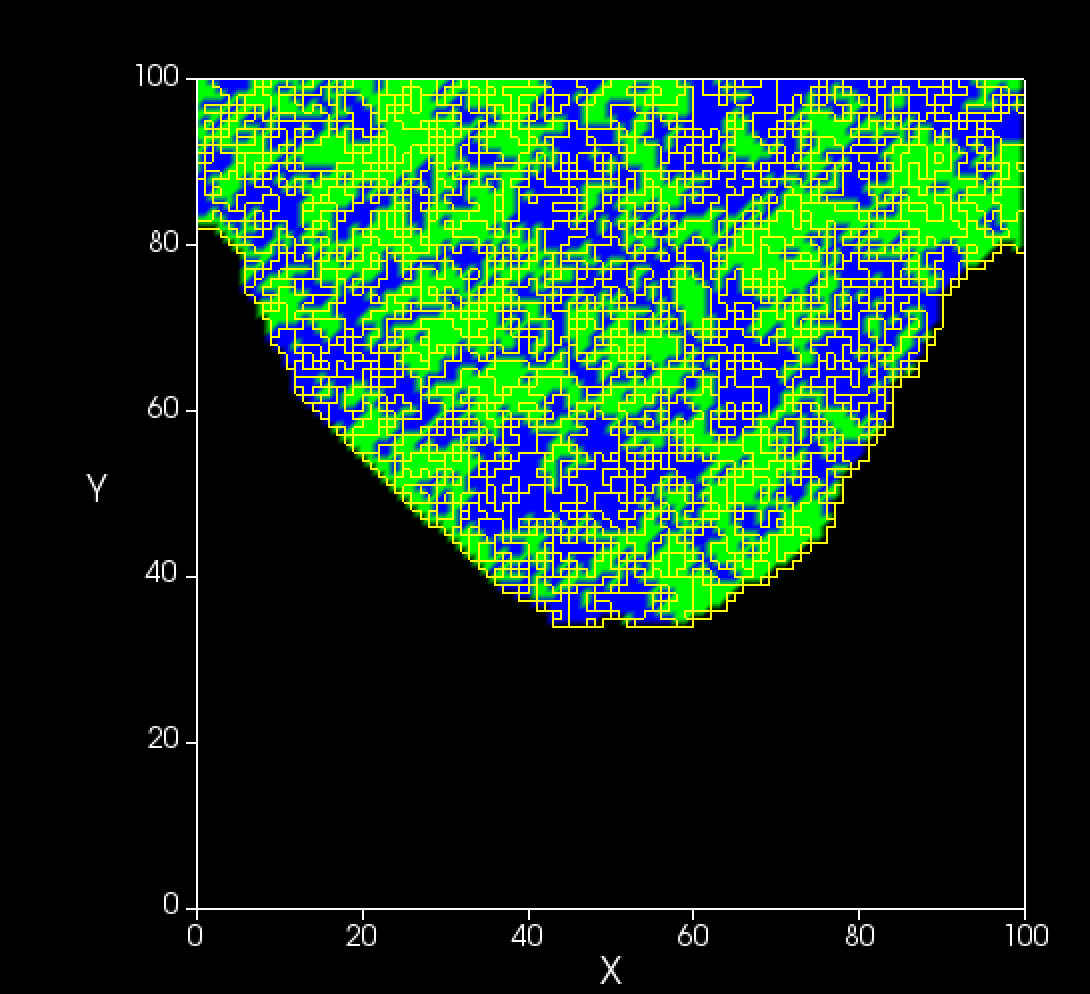
\includegraphics[width=0.5\textwidth]{changing_condensing_0s}
\end{figure}
Next is an iteration of making most 0 and each list item value will be set to 100 in the xml.  This should show off any limiting behaviors.

\subsubsection{NonCondensing, NonCondensing}
value = 100.  This configuration appears to not allow any sorting to take place as the final result appears very random.
    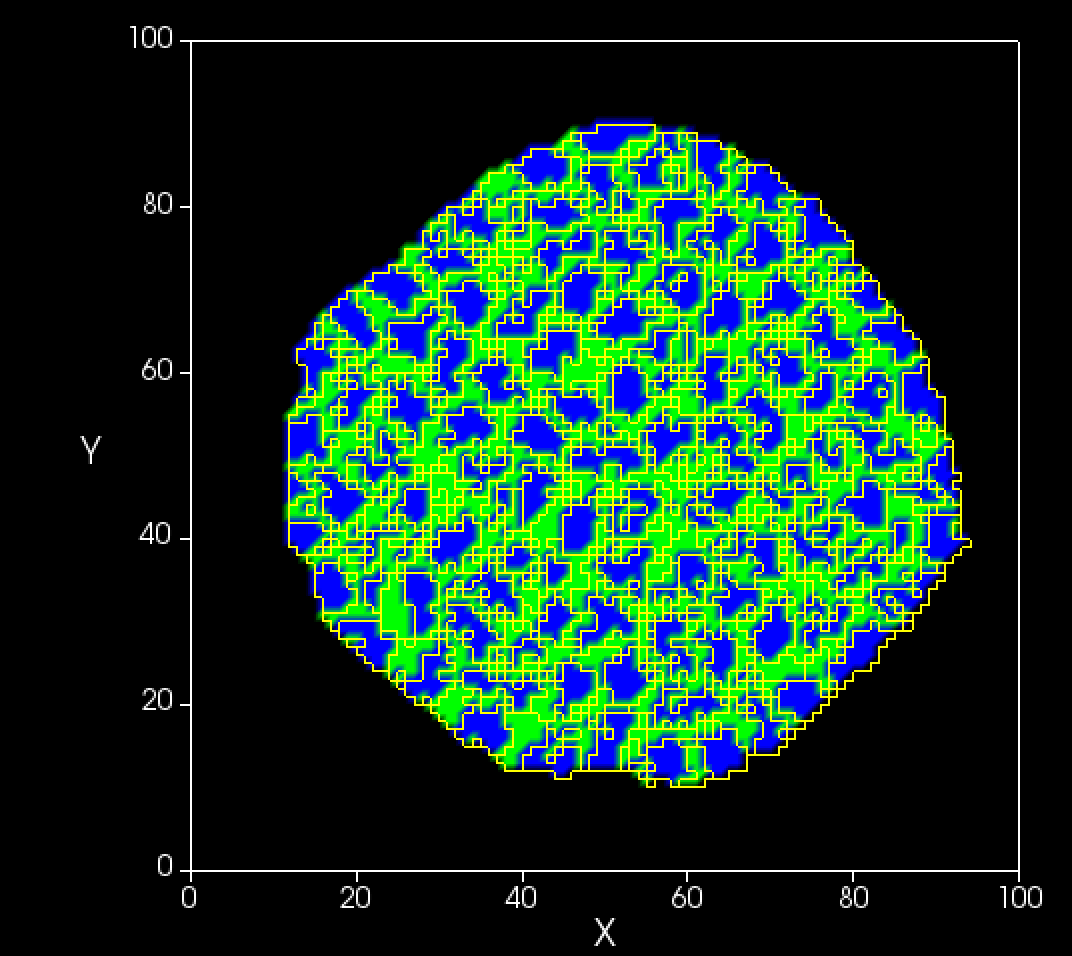
\includegraphics[width=0.5\textwidth]{nC_nC100}
    
\subsubsection{Condensing, Condensing}
value = 100.  This also seems to dissallow sorting and it remains random, but instead of staying in one place it appears to move to the right
    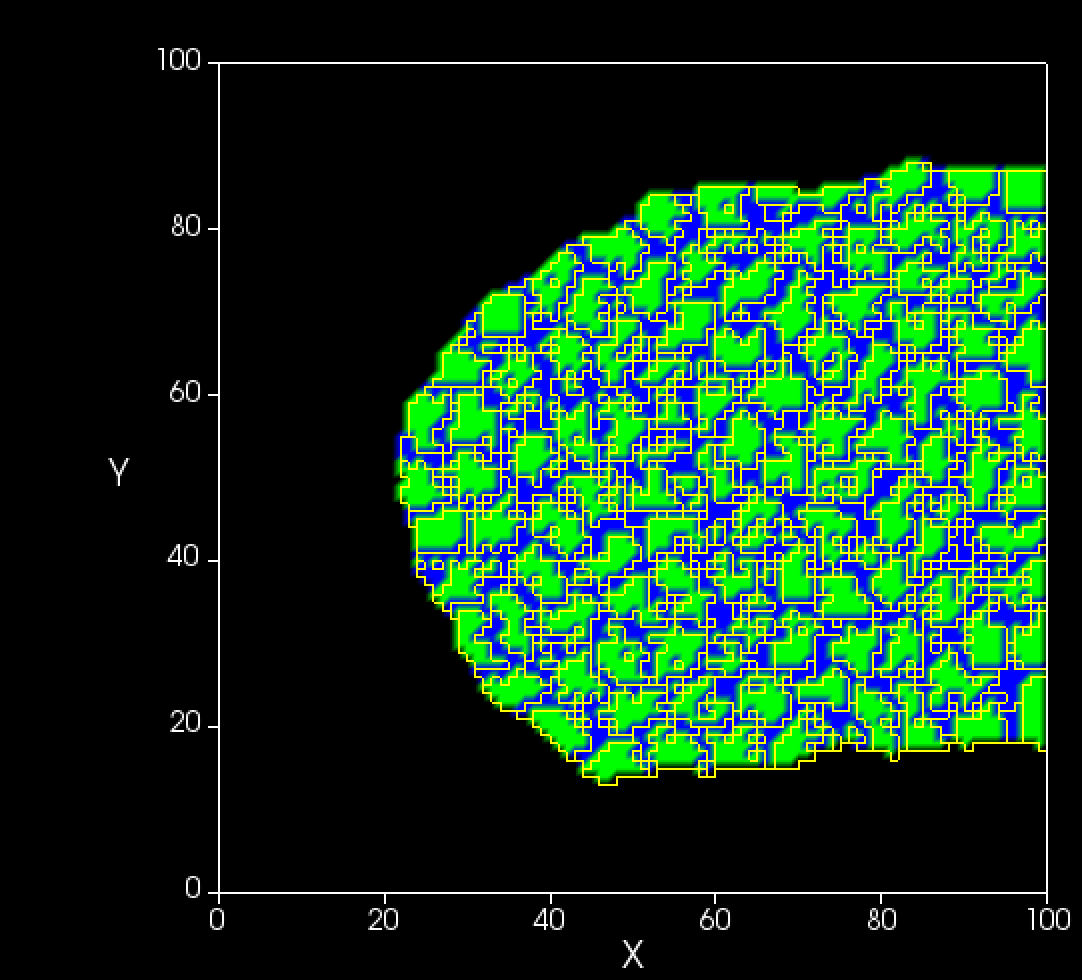
\includegraphics[width=0.5\textwidth]{c_c100}
    
\subsubsection{NonCondensing, Condensing}
value = 100.  This one forces the yellow to stick together and the blue to stick together, but to repel the different colors.
    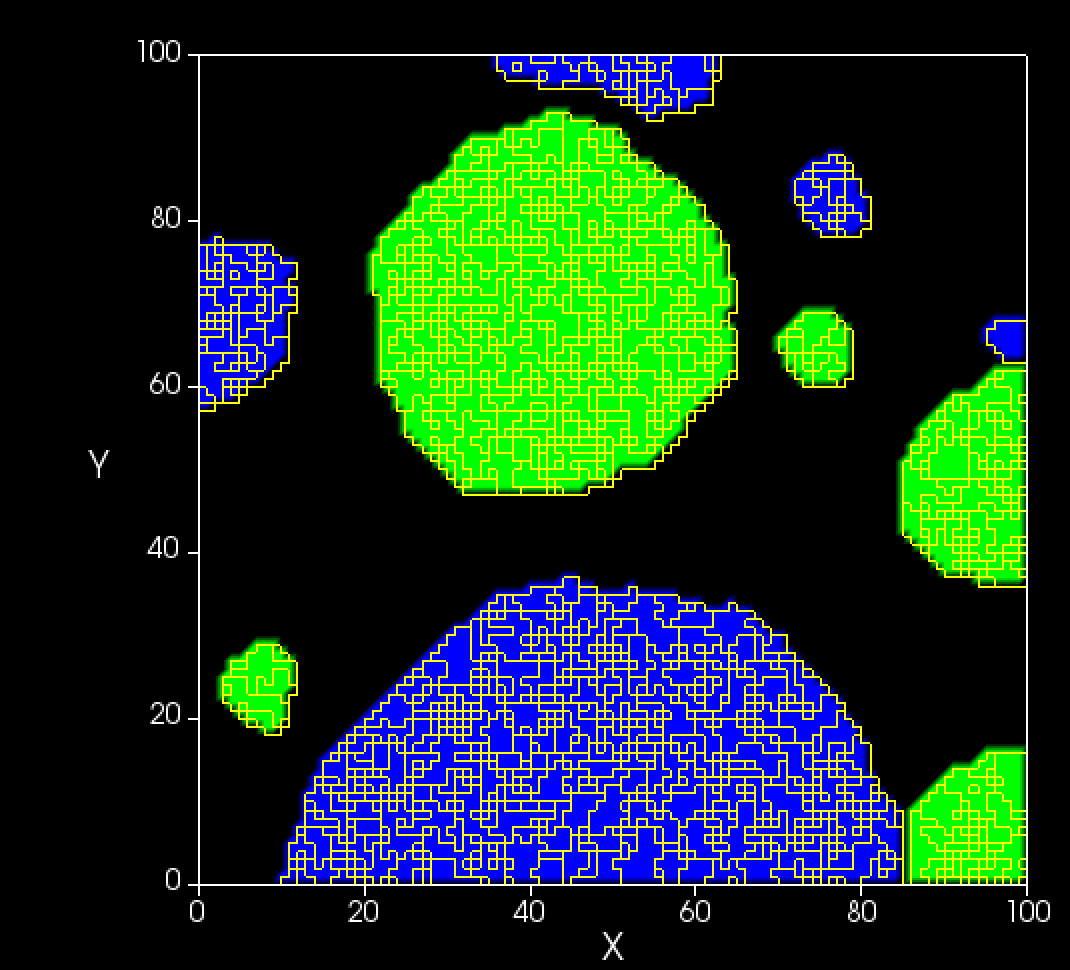
\includegraphics[width=0.5\textwidth]{nC_c100}
    
\subsubsection{NonCondensing, NonCondensing, Condensing, Condensing}
value = 100.  This appears to not have done much to sort it.  It seems to look very similar to the individual state.
    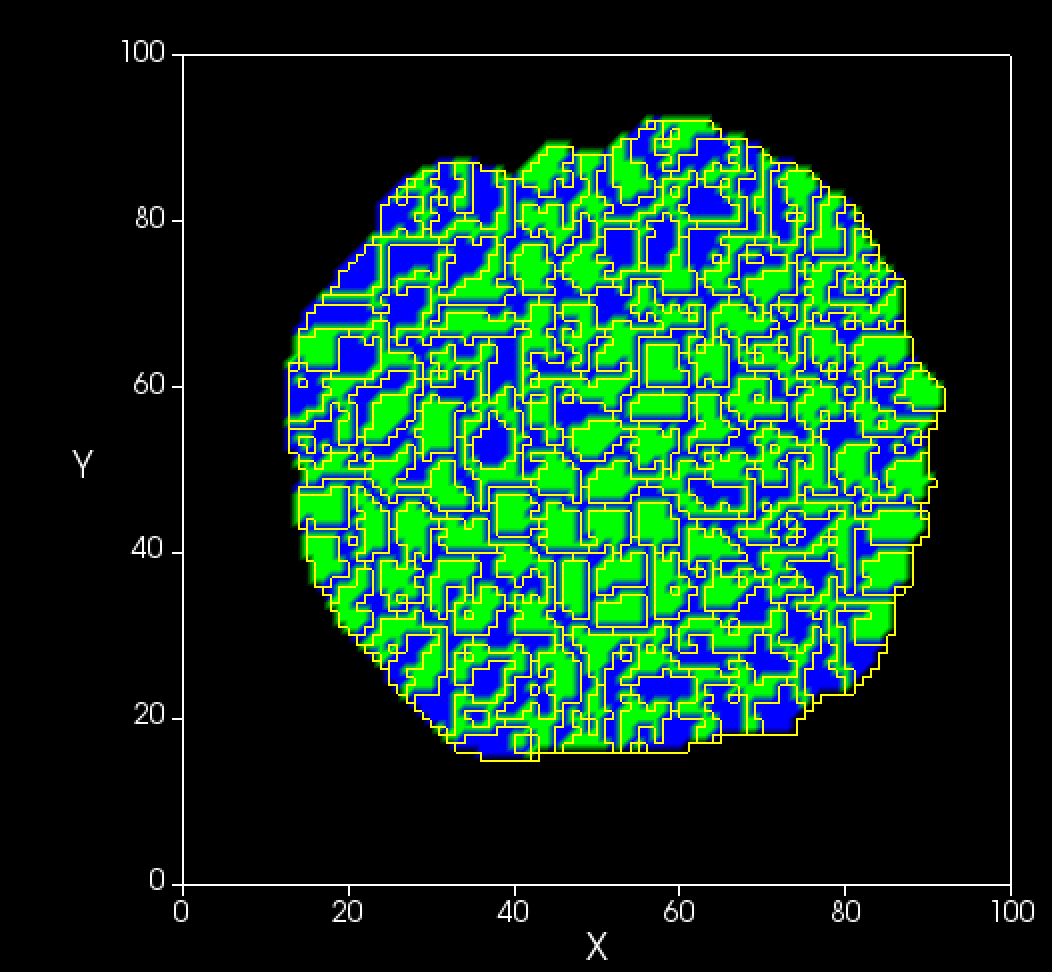
\includegraphics[width=0.5\textwidth]{nC_nC_c_c100}
    
\subsubsection{NonCondensing NonCondensing, NonCondensing Condensing}
value = 100.  This forces the yellow to stick together, but the blue seems to be able to run off on it's own.
    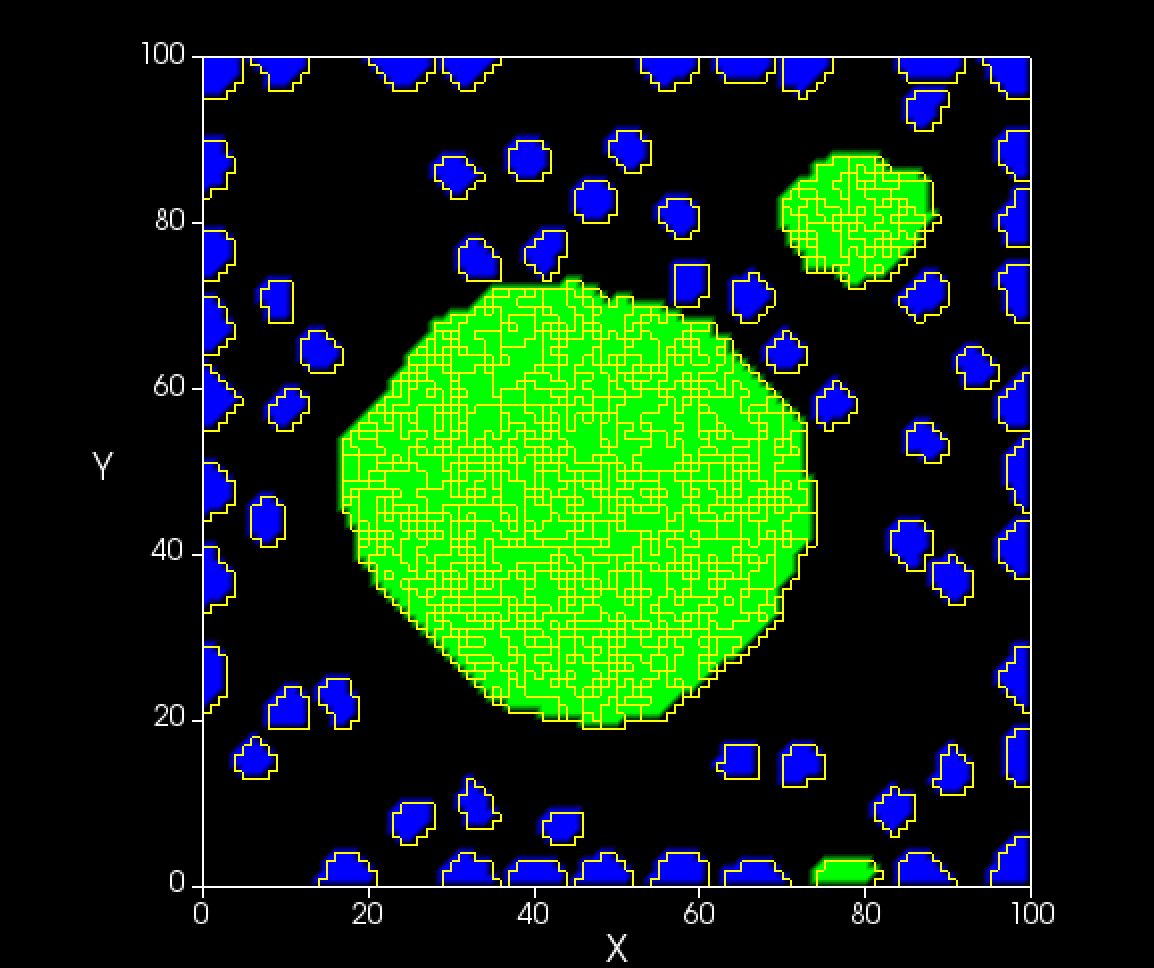
\includegraphics[width=0.5\textwidth]{nC_nC_nC_c100}
    
\subsubsection{Condensing Condensing, NonCondensing Condensing}
value = 100.  From the above i can assume this will make the blue stick together and the yellow to be in small blobs of it's own.  As you can see the assumption is correct, inverted of the one above
    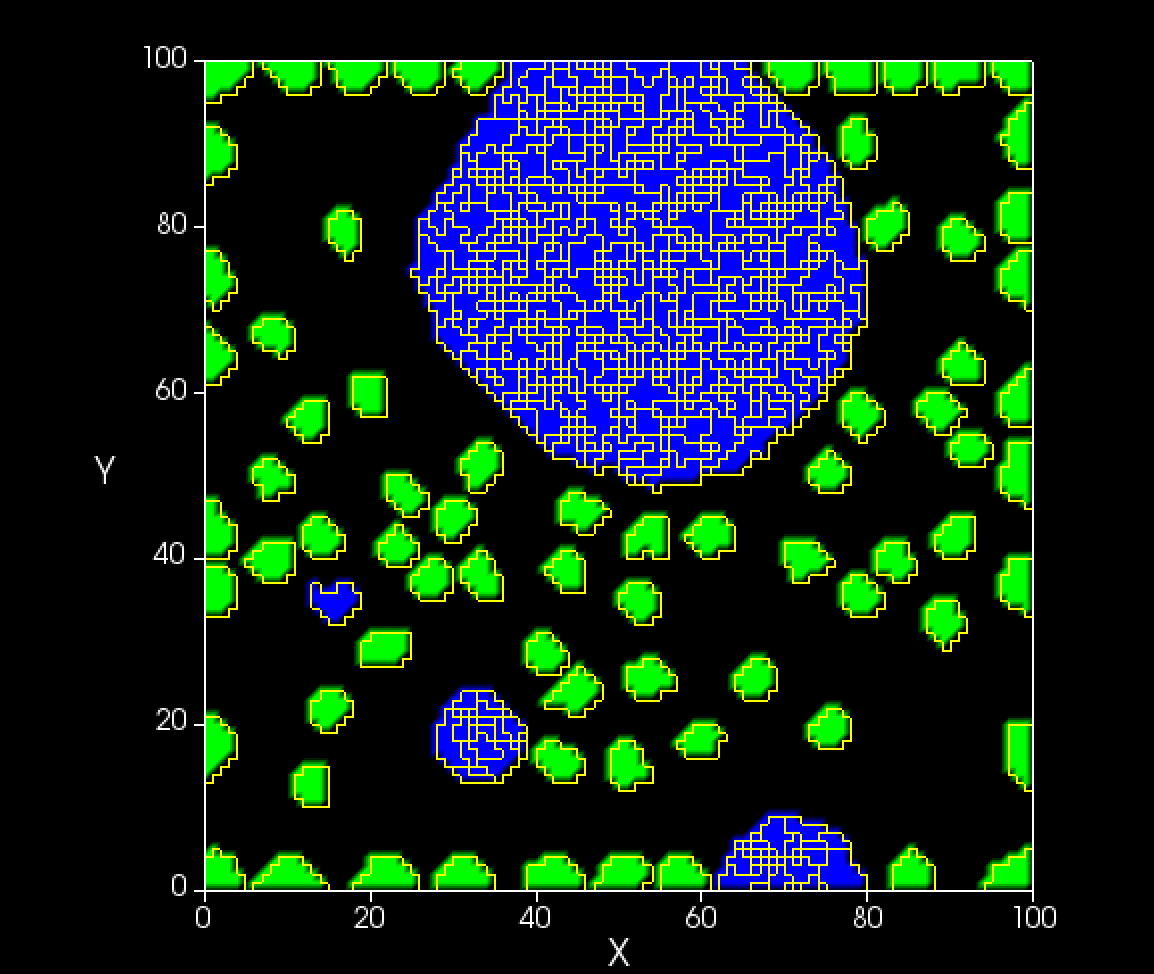
\includegraphics[width=0.5\textwidth]{c_c_nC_c100}

Lastly every one of these to 100 looks like:
This appears that the values are too high to allow them to stick together.
    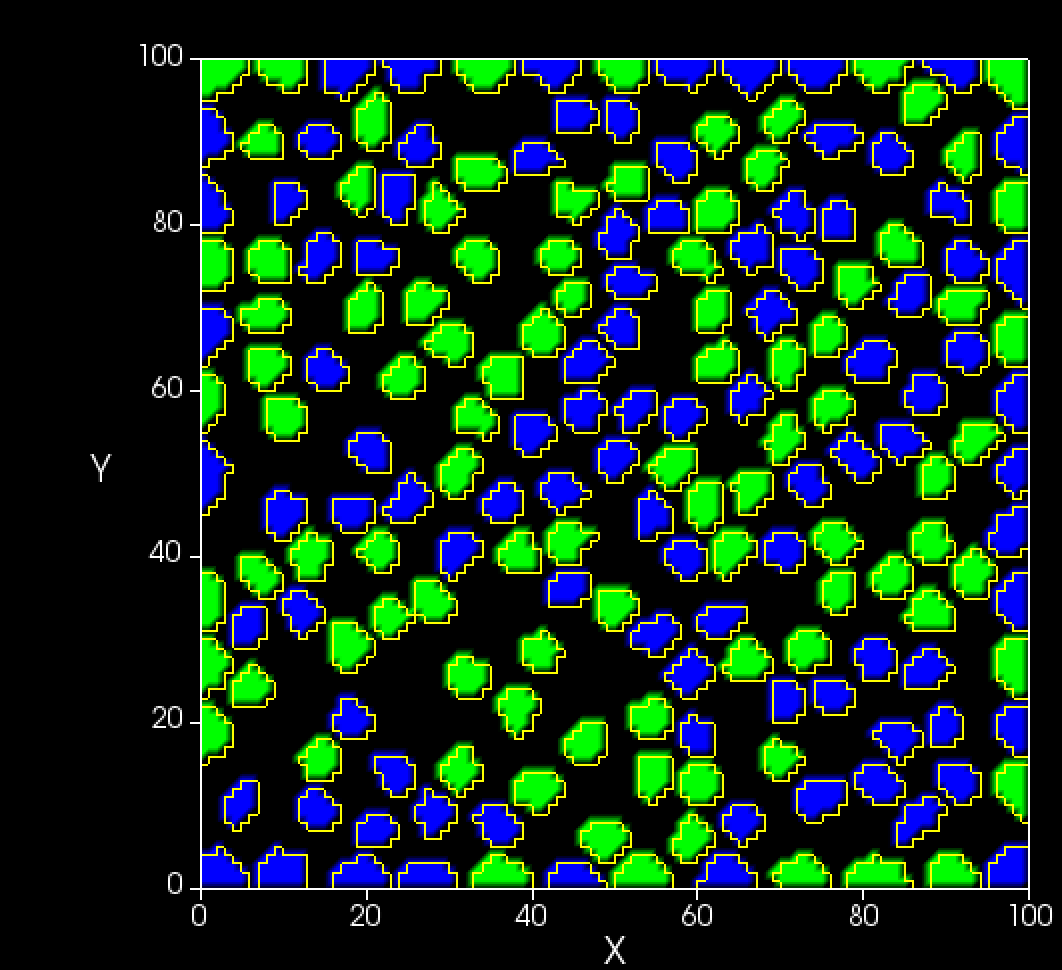
\includegraphics[width=0.5\textwidth]{changing_condensing_100s}

\end{document}
